
%%%%%%%%%%%%%%%%%%%%
%%% INTRODUCTION %%%
%%%%%%%%%%%%%%%%%%%%

%PROBLEM : WHICH INTERACTION TECHNIQUES TO USE WHEN DEVELOPING FOR UI REPLICATION BETWEEN A SMARTPHONE AND A TABLETOP?
%
%SOLUTION : THE PROTOTYPE, SUPPORTED BY BOTH STUDIES

\chapter{Introduction}
\label{introduction}

Modern smartphones are able to support most users' daily computing tasks.
They fit in a pocket, which makes them ultra mobile, and they offer good storage capacities as well as all-around connectivity.
This tendency implies that users have access to personal data and applications at all times.
Smartphones give rise to a new type of computer interaction which is unplanned, spontaneous and on-the-go.
They bring computing to situations where laptops do not fit, such as standing in a crowded train, or walking in the street.
Furthermore, smartphones make it possible to get the most out of unforeseen opportunities, and in particular, they seem to be the ideal tool to support these chance meetings that suddenly turn into constructive collaboration.
However, the size of the smartphone can be a limitation to improvised computer interaction, especially in situations with multiple users. 
\\\\
Tabletop displays, on the other hand, are ideal in social contexts.
They bring computing to a simple piece of furniture, the table.
As such, they present a horizontal interactive surface which multiple users can regroup around, and share a common experience, or conduct parallel activities.
They have been used extensively in museums and galleries, as documented by \cite{Geller:2006:exhibits}, who notes that tabletops encourage a collaborative atmosphere, and provide a tactile experience that reaches even the less computer literate.
As shown in figure~\ref{fig:visitors}, tabletops provide a touch-based experience that is fundamentally different from the traditional desktop metaphor.
A number of HCI studies show that this experience is more natural for the non-technical user, because it removes the mouse-and-keyboard abstraction layer and generates a more direct interaction.

\begin{figure}[htb]
  \centering
    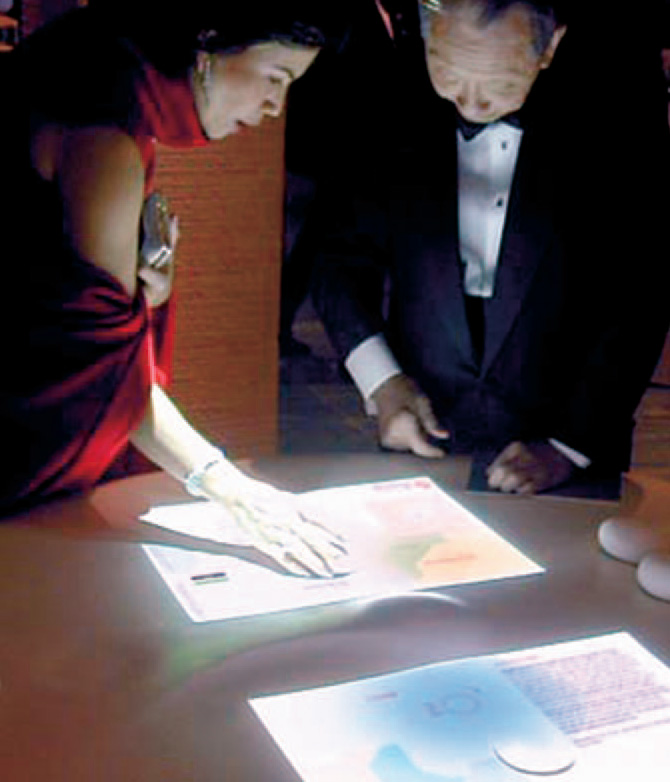
\includegraphics[width=0.4\textwidth]{images/visitors}
  \caption{People using an interactive tabletop exhibit at the Asia Society Museum. Source: T. Geller. Interactive tabletop exhibits in museums and galleries. \emph{Computer Graphics and Applications}, 2006.}
  \label{fig:visitors}
\end{figure}

The first interactive tabletop displays were designed for individual use.
Systems such as the DigitalDesk \citep{Wellner:1993:digitaldesk} aimed at incarnating the desktop metaphor of the personal computer to the common office desk.
However tabletops have a huge potential for collaboration.
Thus, a research branch emerged that focused on \emph{smart rooms}; spaces equipped with various cutting-edge computing devices that can interoperate, to support collaborative work for multiple users.
Tabletops are essential elements of smart rooms, as shown with the InteracTable \citep{Streitz:1999:iland} and the iTable \citep{Johanson:2002:iroom}.

With the emergence of commercial items such as the Microsoft Surface \citep{ms}, tabletops are gradually appearing in public environments such as museums, meeting rooms, public lobbies, bars and restaurants.
They are an ideal platform for spontaneous use and multi-user interactions, and provide a touch-based experience that is similar to the one on most smartphones, which makes them easily accessible to the public.\\
\linebreak
%%% TECHNICAL REVIEW %%%%
%were based on overhead projected output and overhead camera-based input.
%In recent years, however, interactive displays are being commercialized, that are typically based either on computer vision or capacitance.
%
%Capacitive screens are present on the mass market since the iPhone \citep{iphone}, but are now being produced in larger sizes \citep{displax}, \citep{3m}.
%They function by sensing the electrical charge that is produced when a finger interacts with the screen's electrical field.
%This allow for a very precise touch detection, but a drawback is that it does not work with gloved fingers, digital pens or any other objects.
%
%Computer vision can be used in various ways.
%The first Microsoft Surface \citep{ms} as well as the MultiTaction displays \citep{multitouch} function with cameras that detect reflected infrared backlight from objects that are in contact with the screen.
%The main advantage of such solutions is that they can detect not only fingers, but also visual markers and other objects.
%Microsoft has perfected this technology in the latest Surface with PixelSense \citep{pixelsense}, where the individual pixels can detect what touches the screen, thus removing the need for cameras.
%PQ Labs \citep{pq} produces side vision overlays that can provide multi-touch detection to any type of screen, though without the possibility for object detection.
State-of-the-art smartphones boast screen resolutions up to 1280 by 720 pixels, which exceed the naked eye's ability to distinguish separate pixels.
%This implies beautiful graphics with profound and rich colors.
However, a smartphone screen is too small to provide a satisfactory user experience in the presence of multiple users, and when viewing dense content such as text or high-quality images.
Screen sizes for ultra mobile devices only go up to five inches.
Reading a text, consulting a map and viewing images are examples of situations in which small displays present limitations.

An example of graphically dense content is a text of more than a few paragraphs.
The default view of an online blog or a pdf document on a smartphone, is too small for a user to be able to discern single words.
Depending on eyesight, it usually takes two to four zooming gestures to enlarge the text to a size that is conveniently readable.
At this point, the user generally tilts the phone to landscape orientation, in order to give the paragraphs a more natural length.
The screen provides only enough space for five to ten lines of text, which implies the use of successive pan gestures to update the content as the user reads on.
Compared to the simple experience provided by a newspaper or a book, this seems troublesome.

Maps are graphically dense as well.
They present a lot of different information, such as topography, street names and sights on limited space.
To be able to read a street name on a smartphone map application, the user needs to zoom in on the relevant part of the map.
The result is that the user can only view a very limited area.
To be able to relate this area to another location, the user must use a combination of pan and zoom gestures that can be difficult.
In certain cases, the area of interest is simply too vast to be viewed on a smartphone screen.

Viewing pictures on a smartphone is another experience made frustrating by the small screen size.
Modern smartphones take pictures of high quality, and we carry them with us at all times.
However, they are too small for us to conveniently view the pictures that we take, let alone to show them to others.
%However, viewing the images on the device presents serious limitations.
Ideally, showing pictures to a friend implies both persons looking at, and commenting on the pictures simultaneously.
But this is hardly possible on a smartphone.
What typically happens is that the user finds a picture that he wants to show, then hands his phone to the friend, then the friend hands the phone back to the user, who chooses the next picture, and so on.
This process is tiring at best.

Even though smartphones provide multiple opportunities, the aforementioned examples show that a small screen size can cause frustration.
This thesis addresses situations where using a smartphone would be easier if it had a larger screen.
The solution proposed is to make smartphones able to spontaneously integrate with larger displays that are available in the environment.
In particular, the idea is to be able to walk up to a tabletop computer, and with a few easy steps, combine it with one's smartphone.
The result, shown in figure~\ref{fig:tide}, is that the screen of the smartphone is displayed on the tabletop, where it can be enlarged, and conveniently viewed by multiple users simultaneously.

\begin{figure}[htb]
  \centering
    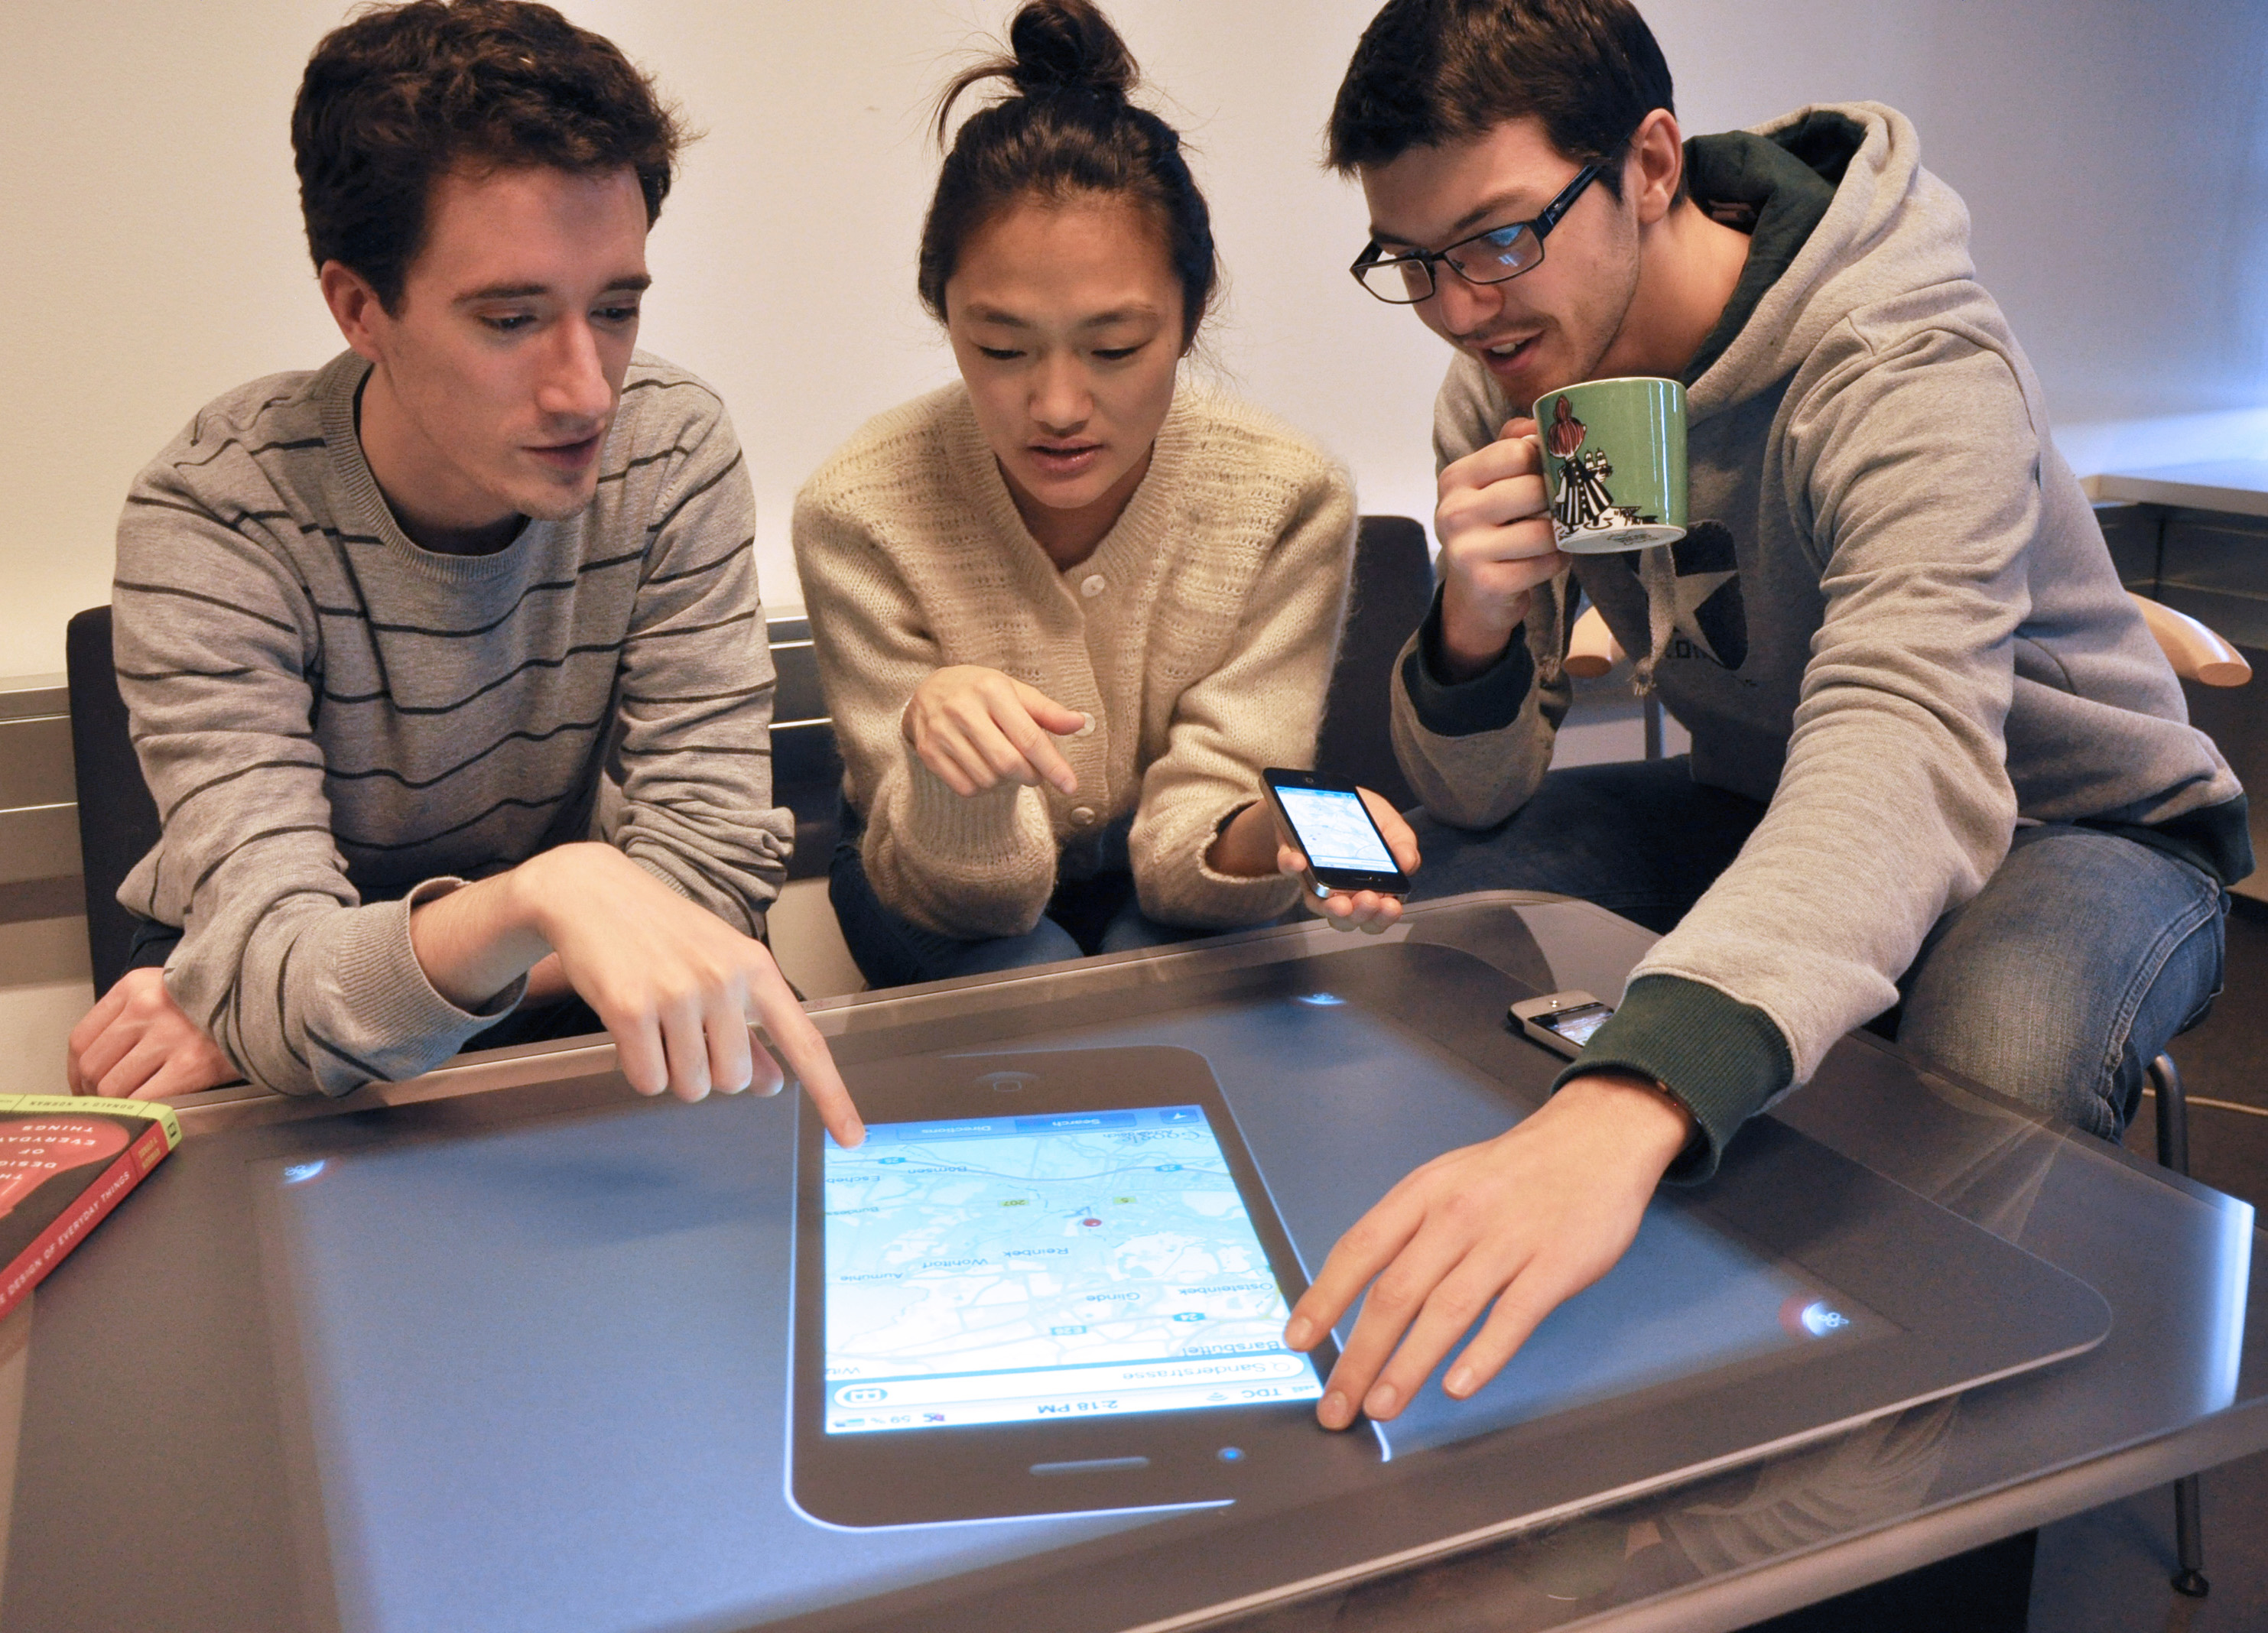
\includegraphics[width=0.6\textwidth]{images/tide456}
  \caption{People using a tabletop to view information on a smartphone.}
  \label{fig:tide}
\end{figure}

%It does so by suggesting a \emph{device composition} approach, that integrates smartphones and tabletops.
%Tabletops are a solution to this problem for several reasons.
%They provide the needed display space, and a touch-based interaction that comes naturally to the typical smartphone user.
%Moreover, they are designed for collocated collaboration, which brings an interesting new dimension to the scenarios discussed above.
%Examples of the possibilities include consulting a map to show a location to a friend, reading and editing a document with a colleague, playing a multiplayer game, or viewing and sharing pictures between smartphones.
To realize this vision, \emph{device composition} can be used, a research approach that can be traced back to the work on smart space technologies and systems such as Augmented Surfaces \citep{Rekimoto:1999:augmentedsurfaces}, \mbox{i-LAND} \citep{Streitz:1999:iland} and the Interactive Workspaces \citep{Johanson:2002:iroom}.
Smart rooms were designed as closed computing environments, so recent efforts have been invested in developing for a more ad-hoc type of device composition, with projects such as Obje \citep{Edwards:2009:obje}, Platform Composition \citep{Pering:2009:platformcomp} and CompUTE \citep{Bardram:2010:compute}.

Tabletops are a central device in the previously mentioned smart rooms, and a recurring element within device composition.
They are an ideal platform for collocated collaboration, as shown with systems such as the MemTable \citep{Hunter:2011:memtable} and SketchTop \citep{Clifton:2010:sketchtop}, that are designed to support the work of technical users.
In recent years, however, tabletops are appearing in public spaces, engaging common users in a more relaxed form of interaction.
\\
\linebreak
Within the context of designing for device composition between smartphones and tabletops, three fundamental challenges must be addressed.

The first one is the pairing procedure responsible for device discovery and connection.
Pairing between unknown devices has been solved in many different ways.
An example that is particularly relevant to this work is the BlueTable \citep{Wilson:2007:bluetable}, an interactive surface that uses Bluetooth to discover and connect to a mobile phone.
The BlueTable improves the process by using computer vision to locate the phone on the table, and verify its identity via the phone blinking an infrared signal.

The second challenge is how to distribute the UI of the smartphone to the tabletop.
Various stable technologies already exist, but recent researchers have chosen to build frameworks from scratch, to allow for a more flexible distribution and sharing of user interfaces between multiple types of devices.
An example of such an approach is XICE (eXtending Interactive Computing Everywhere) \citep{Arthur:2011:xice}, a programming framework that is meant to support a new form of nomadic experience, where users can annex various display servers with their mobile personal devices.

The third challenge is to design a user interaction that suits the purpose of the system.
Different interaction metaphors have been used to extend the UI of smartphones to larger display surfaces, including streaming, replication, expansion, projection and adaptation.
In their recent work on Virtual Projection (VP), \cite{Baur:2012:virtualprojection} built a system where a smartphone can project its UI onto an available computer display.

%Device composition started with SMART ROOMS, and composing various devices, which we want to do in this case.
%But smart rooms were designed as closed environments.
%
%We would like AD-HOC, spontaneous device composition.
%That was addressed by projects like Obje, CompUTE, Platform Composition.
%
%we are interested in mobile to TABLETOP
%- studies on collaboration (but closed environments and technical users)
%- studies on tangible interaction
%
%tabletops emerge in public spaces > non technical users > we focus on standard hardware
%
%we must solve 3 challenges: pairing, UI distributing, user interaction
%
%To combine SP and TT, we need to pair them, which can be done
%with networked protocols or bluetooth
%(but that requires explicit input from user, or CPU/battery intensive continuous sniffing
%SO we use a trigger, that can be:)
%detecting synchronous events
%entering a key into display
%with RFID
%with computer vision to detect
%
%we do it with computer vision detection and networked protocol (Bonjour)
%
%we need a technology to do UI distribution:
%distr data
%distr code
%
%best to distr graphics:
%(we choose VNC in spite of drawbacks > why?)
%
%we need a user interaction
%
%FINISH with how we do differently!

\section{Problem statement}

This thesis addresses the problem of 
%using \emph{consistent} 
designing a composite device between a smartphone and a tabletop computer that allows for \emph{spontaneous interaction}, by focusing on the learnability and ease of use of the system.
\\
\linebreak
It does so by answering the following research questions:
\begin{itemize}
\item What are the requirements for such a system?
\item Which interaction techniques are best suited for this type of system?
\item Can this system be made to run on standard hardware and integrate different smartphone types?
\end{itemize}

\section{Research methods}

To solve the problem at hand, the following research methods were used.
\\
\linebreak
Placing the present work within its research context, 
a comprehensive literary review was made of the prior work related to device composition and surface computing.
In particular, the following aspects of device composition were examined; background, systems integrating smartphones with tabletops, pairing, UI distribution, and user interaction.
The review is presented in Chapter~\ref{relatedwork}.

Following a user-centered approach, a solution design was completed.
The process was divided into the following tasks.
The application's context of use was analyzed based on scenarios and storyboards.
This analysis lead to the definition of the solution requirements.
A series of design options were derived from existing approaches to software design for surface computing.
Design decisions were taken, based on an experiment where end users engaged with low-fidelity prototypes of the system.
The design process, together with the final system design, are presented in Chapter~\ref{design}.

In order to demonstrate the feasibility of the suggested solution, a proof of concept was realized, in the form of an application prototype implemented on the Microsoft Surface tabletop computer, an iPhone 4 and a HTC Legend phone.
The implementation was focused on the user interaction, and the aim of building a system that is easy to learn and use.
The system is described in Chapter~\ref{system}.

An evaluation of the design was conducted by way of a participant-based usability study, that involved the following steps.
The focus of the evaluation was identified, in terms of specific aspects of the system, and the evaluation methods were selected.
A user experiment was designed, that involved a discovery phase, a guided test and a questionnaire.
Participants were recruited, and the experiment was carried out.
Evaluation data was gathered via online forms, then processed, analyzed, and the results were derived.
The evaluation process and results are reported in Chapter~\ref{evaluation}.

\section{Contributions}

This report presents the design, implementation and evaluation of a composite device that integrates smartphones with the Microsoft Surface.
There are three major contributions.
\\
\linebreak
The user-centered design process, presented in chapter~\ref{design} shows, that it is feasible to design a system that is immediately accessible to most users, by focusing on providing a \emph{spontaneous user interaction}.
In order to create an application in which the learning curve is the lowest possible, a lot of focus was given to discover which interaction techniques are familiar to the end users.
To discover the features that would make the system both easy to learn and easy to use, two strategies that are both based on \emph{design consistency} were followed.
The first strategy is to produce a design that is consistent with the smartphone experience.
The aim being to provide a familiar experience to smartphone users, and to help introduce tabletops, which are novel devices, to non technical users.
The second strategy is to realize a product where the design is consistent with the physicality of the devices involved.
Getting inspiration for the tabletop application design from actual tables and from the way people interact with them, the idea is to create an experience that will naturally appeal to end users. 

The design process was based on a careful analysis of the application context, and otherwise focused on how the user will interact with the system.
In order to discover which interaction techniques are most familiar to smartphone users, several user-centered design techniques were used.
The design techniques revolved around the setting up of cooperative design sessions which were based on low-fidelity prototypes.
Figure~\ref{fig:vortex} shows some of the paper prototypes that were used, as well as an early prototype that was used as inspiration for this work.

\begin{figure}[htb]
  \centering
    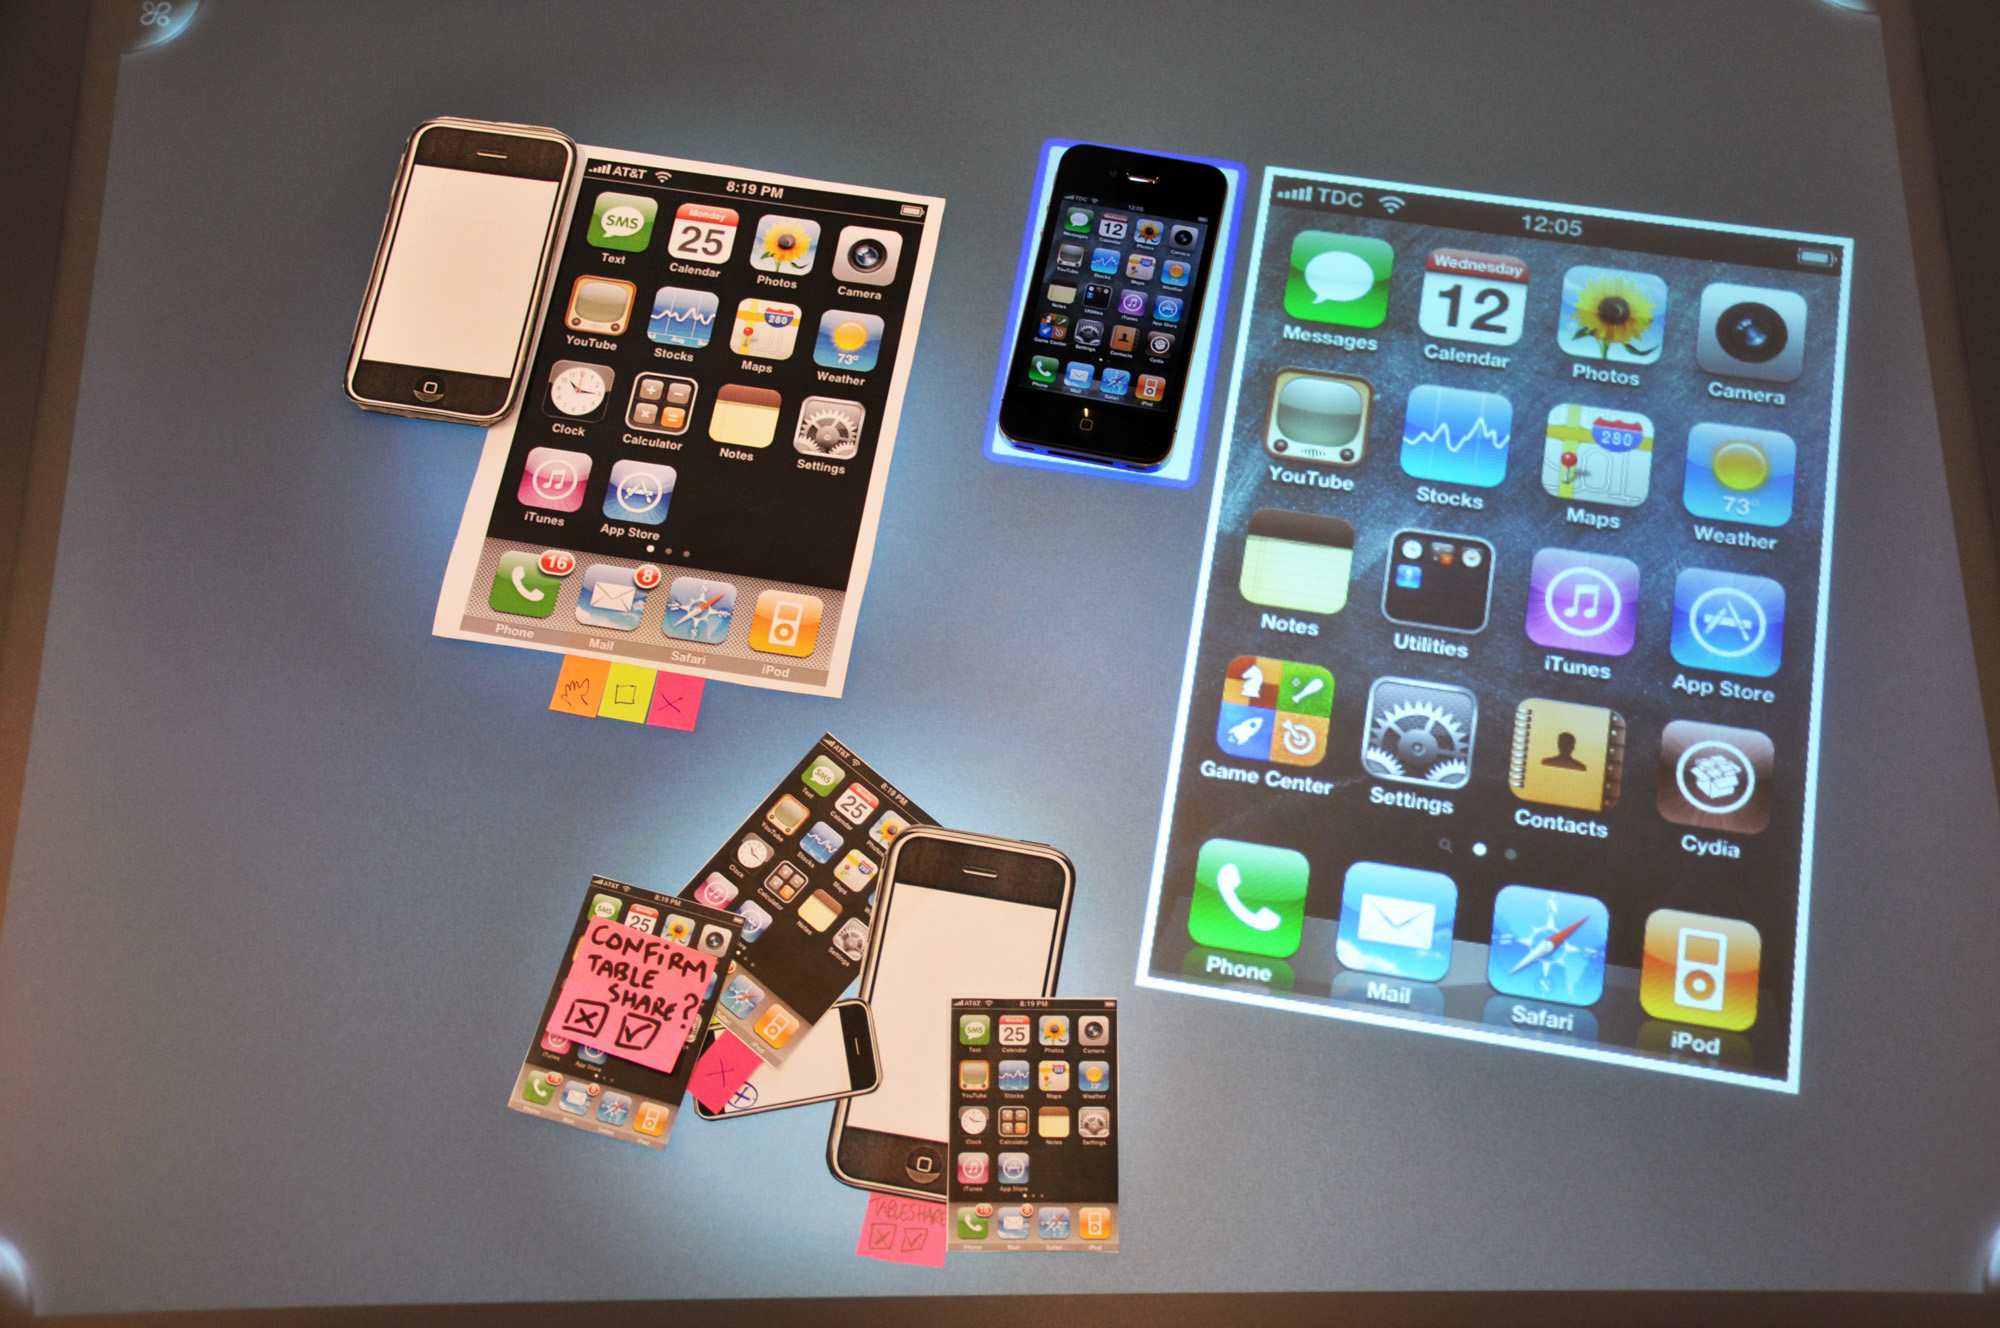
\includegraphics[width=0.7\textwidth]{images/paperprot2}
  \caption{Low-fidelity prototypes and an early digital prototype.}
  \label{fig:vortex}
\end{figure}

By involving end users early in the design process, it could be determined which actions the users would naturally try the first time, they interact with the system.
Also which actions they would not think about.
The result is the design of an application that allows the user to walk up to a tabletop, and easily transfer the content of his/her smartphone's screen to the interactive surface for an improvised experience.
The replicated screen is surrounded by a frame that can be intuitively manipulated to control the size, position and rotation of the remote user interface.
Multiple interaction techniques were used to ensure that the application features are both easy to discover and efficient.
\\
\linebreak
The implementation of the proof-of-concept application called \emph{TIDE (Tabletop Interactive Display Extension)} is presented in chapter~\ref{system}.
It shows that it is feasible to implement a system on the Microsoft Surface \citep{ms} that can connect to a smartphone and extend its user interface.
TIDE works by way of UI replication, it displays a copy of the smartphone's screen on the tabletop, and relays any touch input from the tabletop to the smartphone.
Multiple simultaneous smartphones can be used, and the currently supported models are iPhone 4 (iOS \citep{ios}) and HTC Legend (Android \citep{android}).
However, TIDE was designed to be extended to support other models as well.
A short descriptive video as well as source code is available online, the link is included in appendix~\ref{video}.

TIDE uses shape recognition to detect smartphones that are in contact with the surface, thus triggering a pairing procedure.
The connection is established quickly and securely.
The smartphone can be disconnected and reconnected easily, enabling the application to support short successive interactions.
Shape recognition is based on computer vision techniques.
The computer vision algorithms are used to detect specific device features, by processing and analyzing the raw visual input provided by the Microsoft Surface camera-based system.
This technique is also used to track the location of the smartphones during the application session, enabling the application to know where the devices are, and when they are removed.
At the core of the system is the replication of the smartphone UI on the tabletop.
The replication is done with the VNC protocol \citep{Richardson:1998:vnc}, due to its stability and availability on many platforms.
The client is integrated to the TIDE application, while the server relies on a third-party application installed on the smartphone.
The mirrored UI is referred to as \emph{replicated UI} in the rest of this report.
It is contained by a visual frame that will be referred to as \emph{surface UI}, which implements all the UI elements that allow the user to manipulate the replicated UI on the tabletop.
%An overview of the TIDE user interface is given in figure~\ref{fig:alone}: user, smartphone, tabletop, surface UI and replicated UI.
%
%\begin{figure}[htb]
%  \centering
%    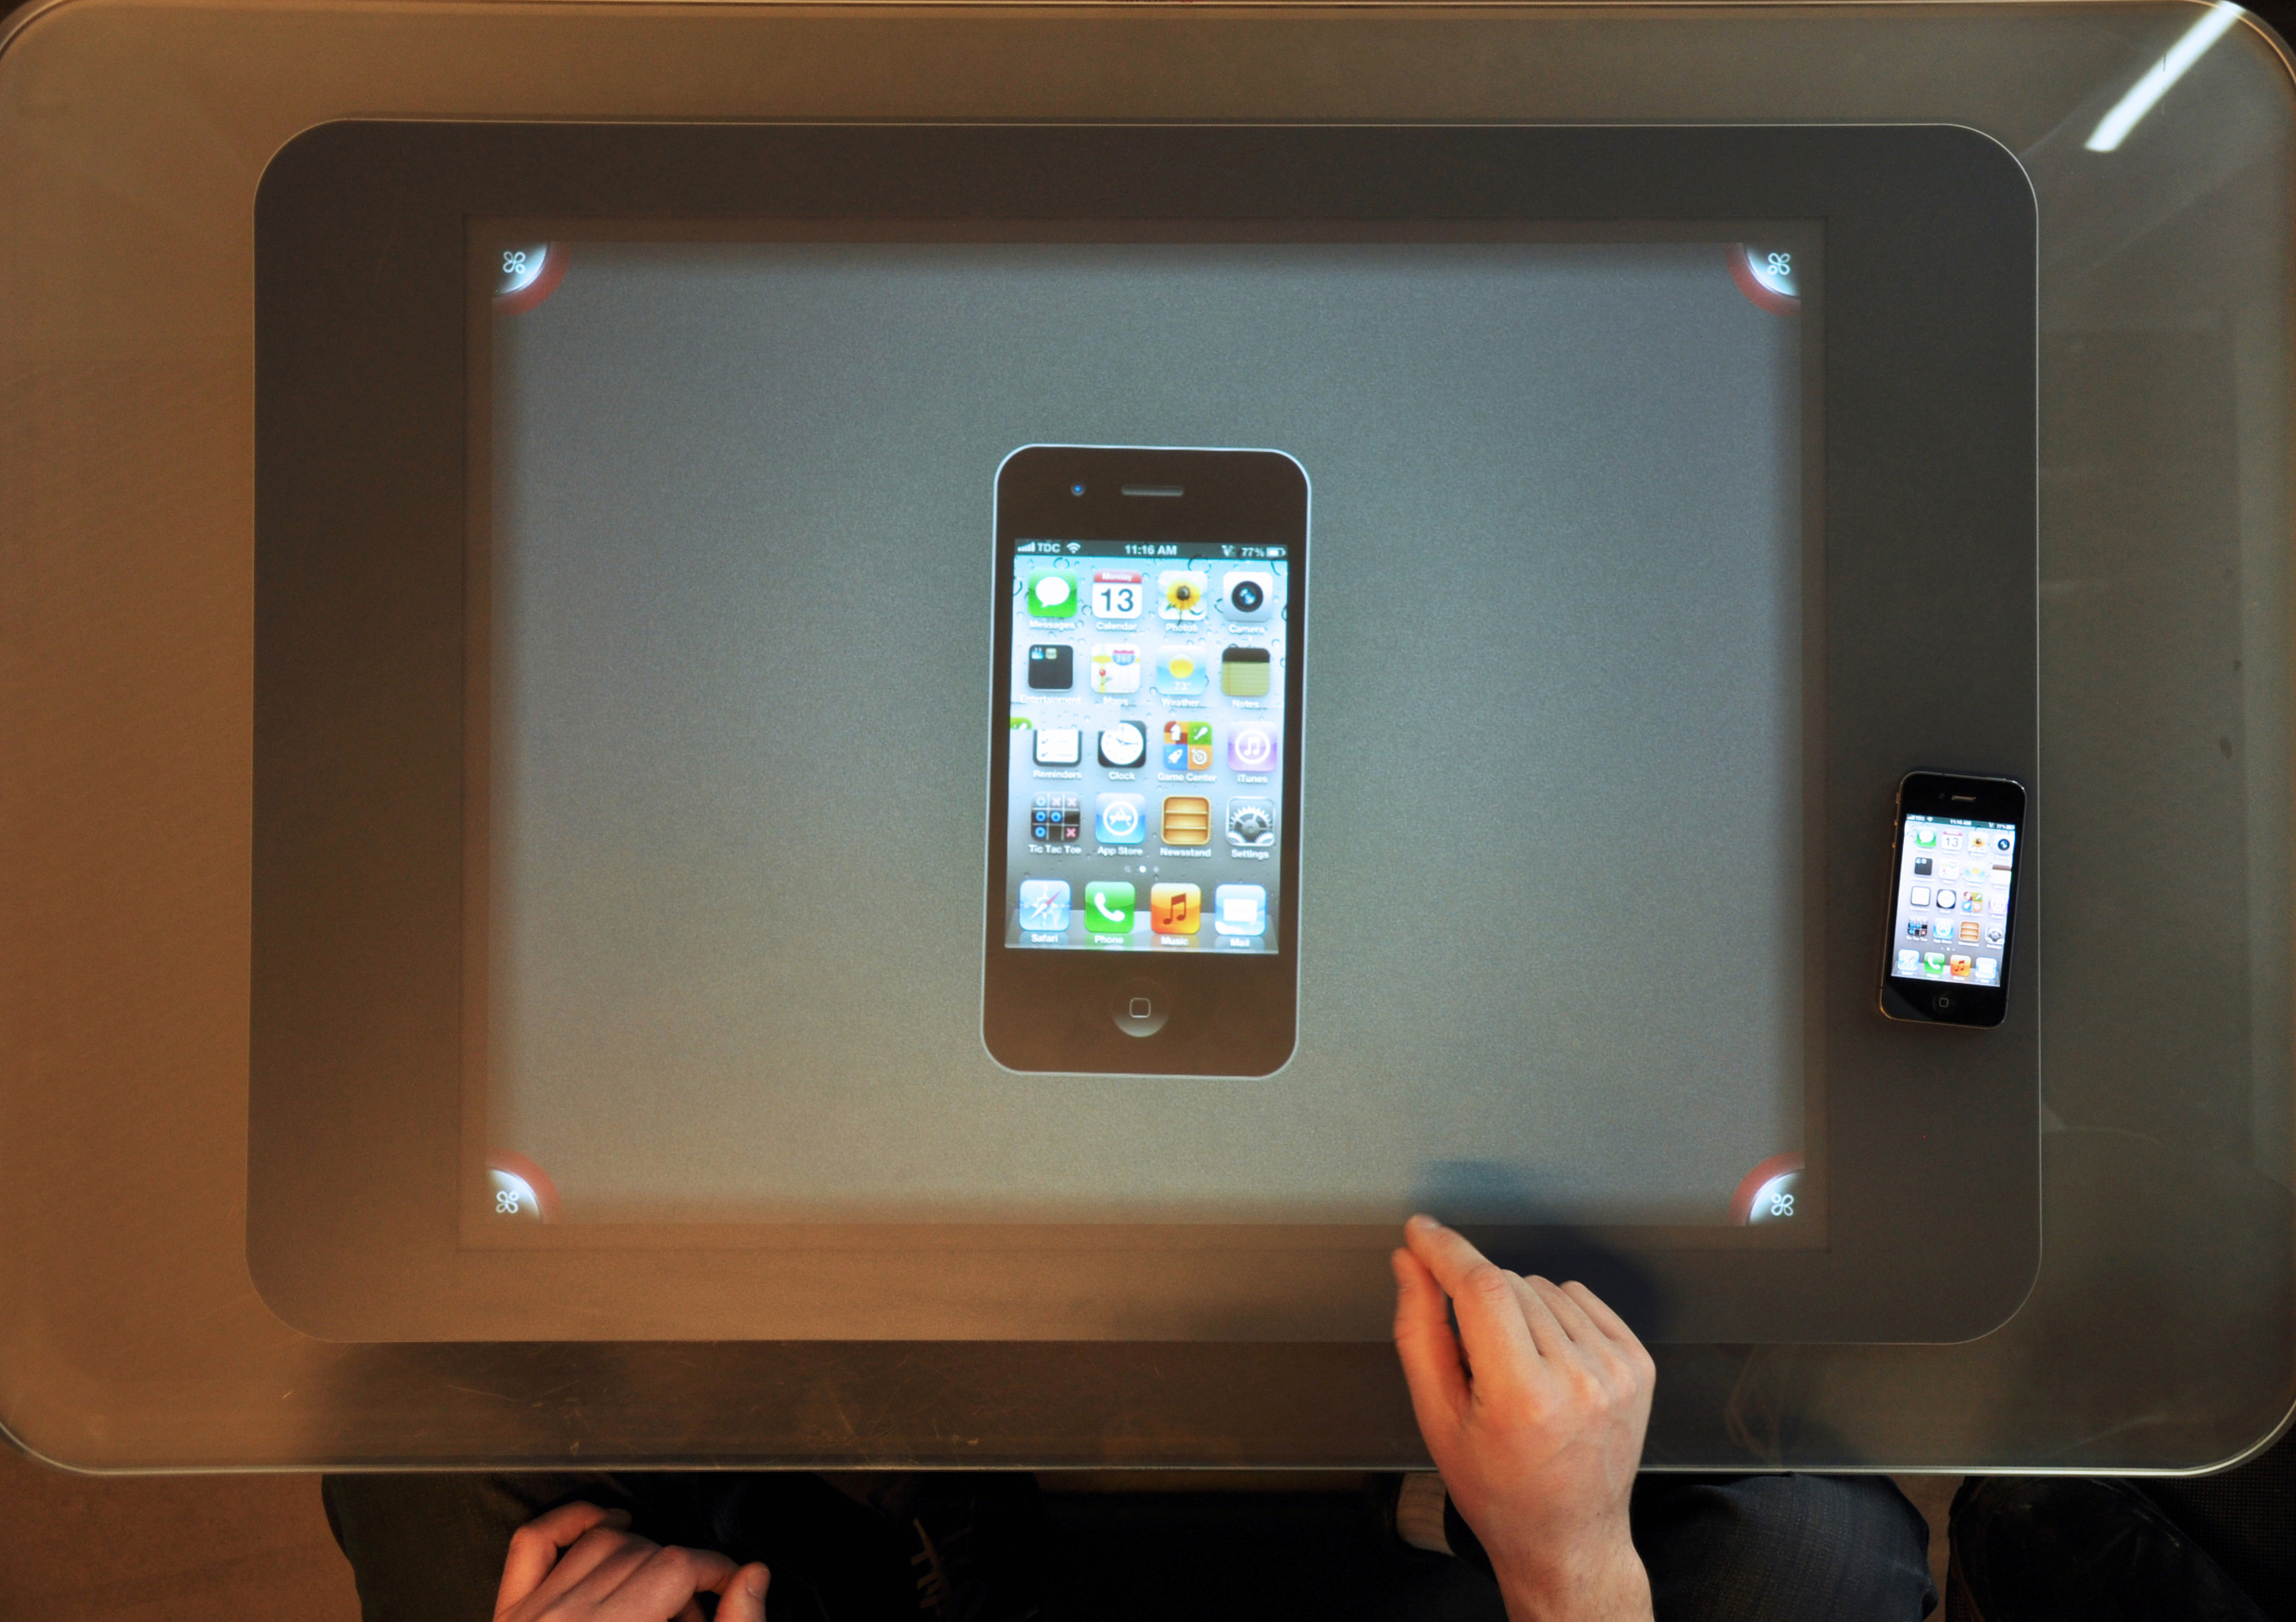
\includegraphics[width=0.6\textwidth]{images/alone}
%  \caption{A person using TIDE with an iPhone.}
%  \label{fig:alone}
%\end{figure}

The surface UI has the same visual aspect as the physical casing of the smartphone, thus providing a natural user interaction.
By using the Presentation layer of the Microsoft Surface SDK, the surface UI implements features that allow the replicated UI to be manipulated via touch-based gestures.
\\
\linebreak
The final contribution is the evaluation of the TIDE prototype presented in chapter~\ref{evaluation}, which shows that the user-centered approach lead to the design of a composite device that provides a spontaneous user interaction.
The system was evaluated by way of a participant-based usability study that confirmed that it is highly learnable, easy to use and useful in specific contexts.
The usability study took the form of an experiment where thirteen volunteers used the application, as shown in figure~\ref{fig:368}.

\begin{figure}[htb]
  \centering
    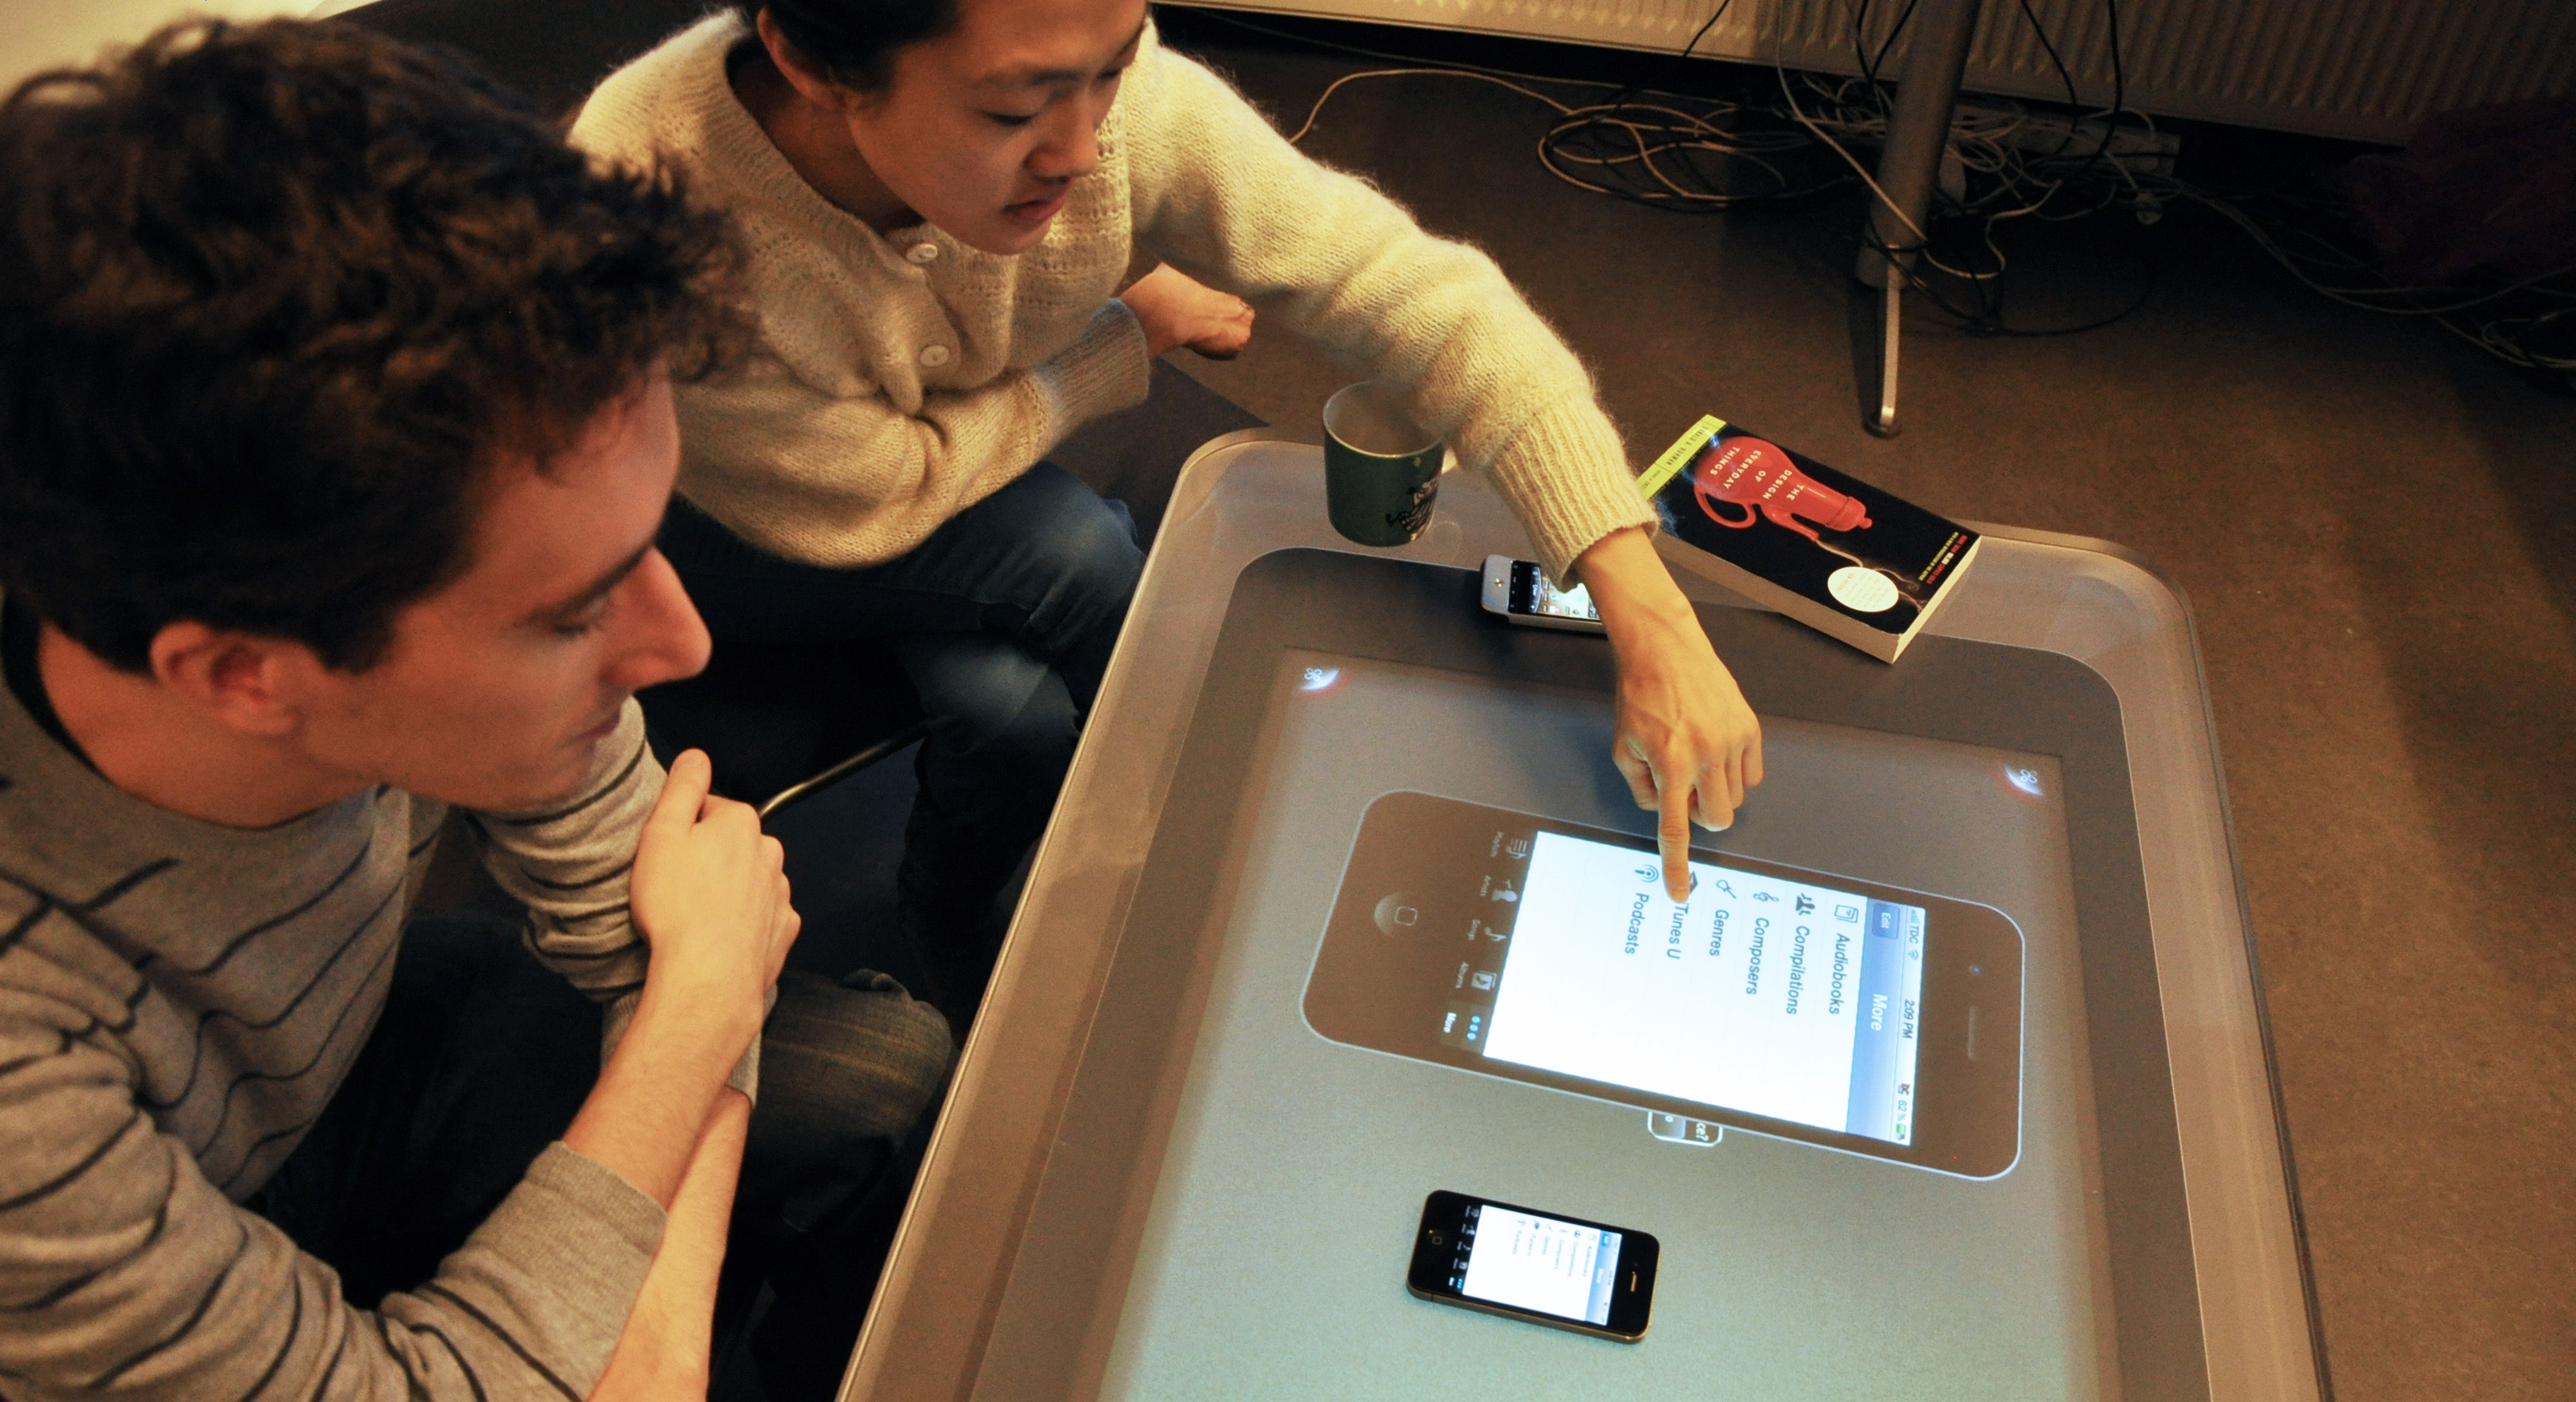
\includegraphics[width=0.7\textwidth]{images/368}
  \caption{End users trying the TIDE prototype.}
  \label{fig:368}
\end{figure}

The participants went through an exploratory test, a semi-controlled one, then answered a carefully designed questionnaire. The experiment generated qualified data, whose analysis helped determine which interaction techniques make TIDE easy to learn, which make it easy to use, and in which contexts TIDE is useful.
The results show that the touch-based techniques for shape manipulation come naturally to most users.
An example being the action of enlarging the surface UI by touching both sides with two fingers and pulling apart.
Other techniques that turned out to be familiar to most users are techniques that are part of common IT knowledge due to the user's cultural background, an example of which is the double tap.
However, the results do not confirm the idea that the form of the tabletop can inspire interaction techniques that seem intuitive to the user, such as dragging a UI element to the edge of the table as one could with a real document.

Lastly, the participants' answers to the questionnaire show that the system is useful when performing specific activities, including browsing internet, looking at pictures and playing games.
However, users do not feel comfortable using the system in a public environment, due to the open aspect of the tabletop display.

%\section{Thesis overview}
%
%Chapter~\ref{relatedwork} presents a literary review of the research that constitutes the background to this work, and the theoretical work on which the design approach is based.\\
%Chapter~\ref{design} describes the process that lead to the design of the TIDE prototype.\\
%The system itself is presented in Chapter~\ref{system}, and its evaluation by way of a usability study in Chapter~\ref{evaluation}.\\
%Chapter~\ref{discussion} is a discussion that addresses the results and lessons learned throughout this process, and brings suggestions for future work.\\
%Chapter~\ref{conclusion} concludes the report.

% solution : using tabletops as UI peripherals
%%%%%%%%%%%%%%%%%%%%%%%%%%%%%%%%%%%%%%
%The specificity of tabletops raises the question of how to interact with them on an everyday basis.
%Recent development initiatives tend to answer this question by regarding tabletops as yet another computational platform, requiring its own software.
%With this project, we explore a different approach to integrating tabletops in our environment, namely by using them only as UI peripheral, providing touch-based input and graphical output to the devices that we already have.
%Exploring this path is supported by three important factors.
%First, most users already own computing devices, such as laptops or smart phones, with tailor-made applications and local storage, and might be less prone to use an additional device if it requires management (updates, backups, synchronizations, etc) and the purchase of applications.
%Second, tabletops are embedded in the environment and as such can be expected to be shared devices.
%Using them as simple graphic peripheral would allow to avoid the traditional desktop/laptop issues related to user profiles, privacy and data integrity.
%Finally, as embedded devices, it is reasonable to expect tabletops to have good networking capabilities.

% device composition
%%%%%%%%%%%%%%%%%%%%%%%%%%%%%%%%%%%%%%
%Device composition focuses on getting the most out of various computing entities, by making them work together and function as one, as seen in \cite{Bardram:2010:compute}.
%This project explores device composition for UI integration between tabletops and mobile devices, focusing on seamless user experience and implicit human computer interaction as defined by Schmidt in \cite{Schmidt:2000:implicit}.

% UI integration metaphors
%%%%%%%%%%%%%%%%%%%%%%%%%%%%%%%%%%%%%%
%UI integration can happen in several different ways:
%\begin{itemize}
%\item{\emph{UI transfer} (mirror): the tabletop `takes over' and displays the UI of the connected device.}
%\item{\emph{Dual view}: the tabletop display becomes secondary screen space for the connected device.}
%\item{\emph{UI nesting}: the connected device is physically located on the tabletop, and its UI is extended to the additional screen space around it.}
%\end{itemize}

% challenges
%%%%%%%%%%%%%%%%%%%%%%%%%%%%%%%%%%%%%%
%Following is an open list of problems that we will address in order to achieve device composition by means of implicit interaction.
%\begin{enumerate}
%\item{\emph{Setup}: How is a device enabled for integrating with a tabletop?
%The setup should be simple, to be performed only once by non-technical users.
%An initial survey of possible solutions points towards the use of tagging mechanisms and/or camera-based object recognition.}
%\item{\emph{Discovery}: How do the tabletop and the device discover and communicate with each other?
%How do we solve the issues of discovery, handshake, network connectivity, and encryption mechanisms to ensure privacy?}
%\item{\emph{UI transfer}: Given the computational constraints of mobile devices, how can the UI transfer be efficiently implemented so as to support native applications and guarantee a seamless user experience?}
%\item{\emph{Input}: How can the users interact with their applications on the tabletop (touch and other peripherals)?}
%\item{\emph{Interaction Design}: What means of interaction are best-fitted for the tabletop-based systems that we propose to develop?
%How can we best adapt to public/private uses and single/multiple users?
%How can we take advantage of the larger interaction surface?}
%\end{enumerate}

